%----------------------------------------------------------------------------------------
%	Inställningar och dokumentkonfiguration
%----------------------------------------------------------------------------------------

\documentclass[paper=a4, fontsize=11pt]{report} % A4-sida och 11 punkters fontstorlek

\usepackage[T1]{fontenc} % 8-bitarskodning som har 256 glyfer
\usepackage[english]{babel} % Svenskt språk(ändrat till engelska)
\usepackage[utf8]{inputenc} % För svenska tecken
\usepackage{dtklogos} % Logos
\usepackage{wallpaper} % Bakgrundsbild
\usepackage{fancyhdr} % Specialsidhuvud och sidfot
\usepackage{enumerate} 
\usepackage{hyperref}
\usepackage{textcomp}
\usepackage{xifthen}% provides \isempty test
\pagestyle{fancyplain} % Använd sidhuvud och sidfot på alla sidor
\fancyhead[L]{Laboration 1 -- 1DV020 -- VT15 -- Server administraion I} % Titel till vänster i sidhuvud
\fancyhead[C]{} % Tomt i mitten
\fancyhead[R]{} % Tomt till höger
\fancyfoot[L]{{\color{gray}\textcopyright \ 2015 Jacob Lindehoff, Kristoffer Schill}} % Tomt till vänster
\fancyfoot[C]{}  % Tomt i mitten
\fancyfoot[R]{\thepage} % Sidnumrering till höger i sidfoten
\renewcommand\thesection{\arabic{section}} % Section beter sig som i dokumentklassen article

\newcommand{\win}[1]{Microsoft Windows Server\ifthenelse{\isempty{#1}}{}{ #1}}
\newcommand{\gui}[0]{``Server with a GUI''}
\newcommand{\core}[0]{Windows Server Core}
%----------------------------------------------------------------------------------------
%	TITLE SECTION
%----------------------------------------------------------------------------------------
\newcommand\BackgroundPic{
    \put(-50,-50){
    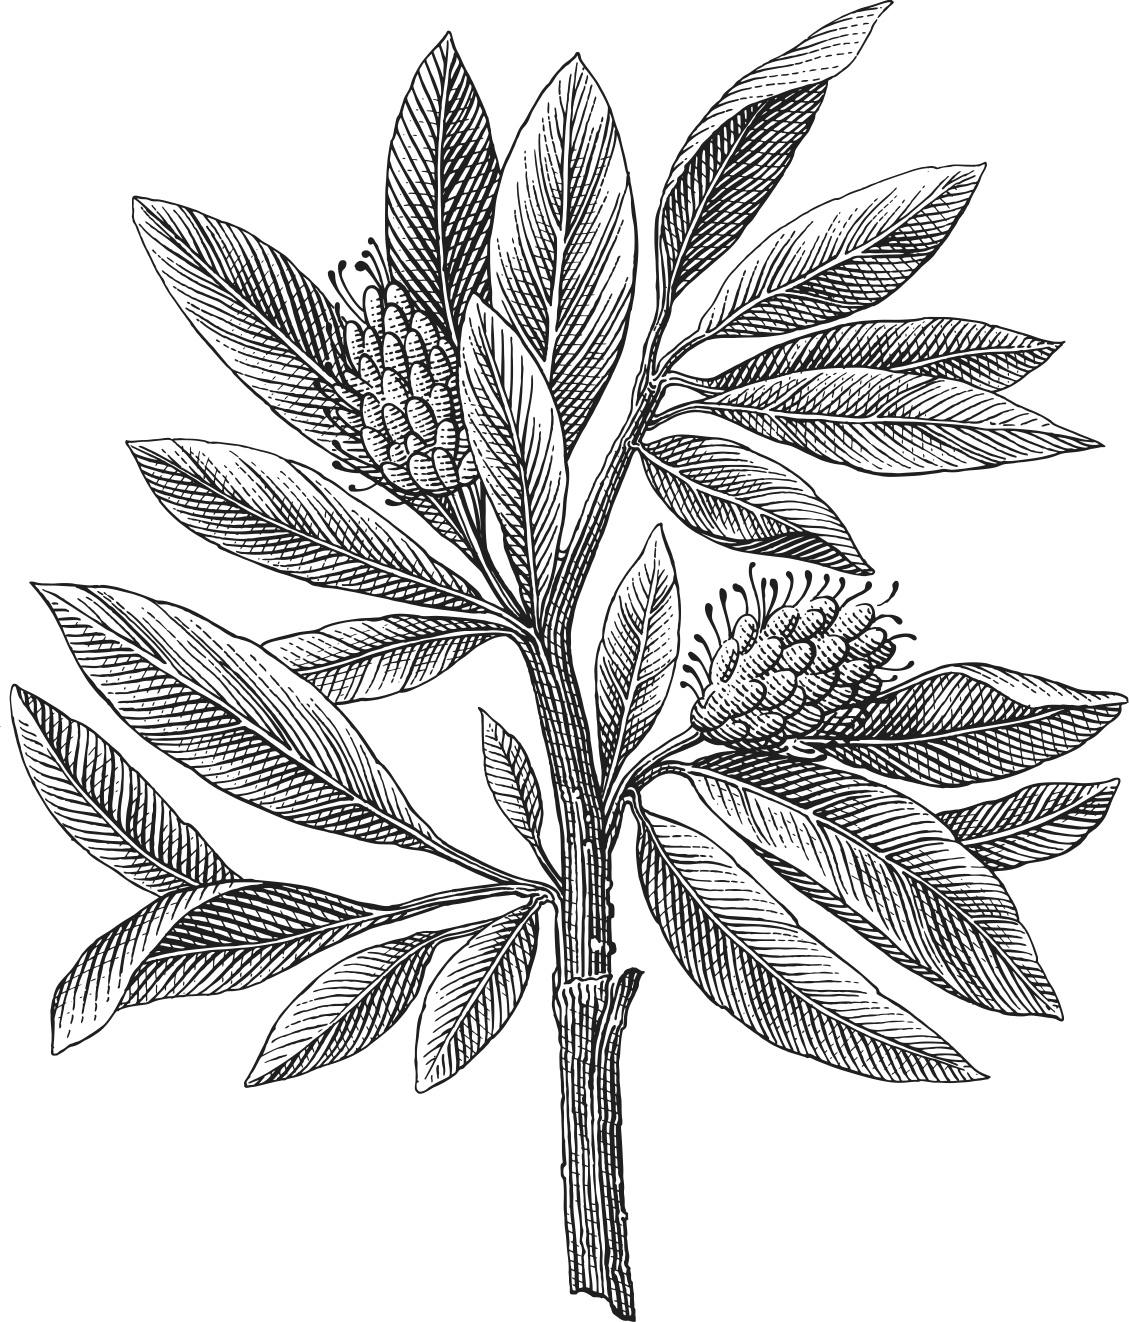
\includegraphics[keepaspectratio,scale=0.65]{lnu_etch.png} % Bakgrundsbild
    }
}
\newcommand\BackgroundPicLogo{
    \put(15,700){
    
\includegraphics[keepaspectratio,scale=0.10]{logo.png} % Logga i vänstra hörnet
    }
}

\newcommand{\horrule}[1]{\rule{\linewidth}{#1}} % Skapa hortisontell linje

\title{	\vspace{-10cm}
    \normalfont \normalsize
    \textsc{Linnéuniversitetet} \\ [25pt] % Universitetes namn
    \horrule{0.5pt} \\[0.4cm] % Tunn linje högst upp
    \huge Laboration 1\\ % Arbetes titel
	\large \textcolor{gray}{1dv020 -- Serveradministraion}
    \horrule{0.5pt} \\[0.4cm] % Tunn linje längst ner
}

% \author{Jacob Lindehoff} % Författarnas namn

\date{\normalsize\today} % Dagens datum

\begin{document}
\AddToShipoutPicture*{\BackgroundPic} % Lägger in backgrundsbild på första sidan
\AddToShipoutPicture*{\BackgroundPicLogo}
\maketitle % Skriv ut titeln
\noindent % Tabba inte in på första meningen

%------------------------------------------------
%	Introduction
%------------------------------------------------
\section{Introduction}

You are an IT-technican on a small newly founded company and the board have given you the task to install the company's first servers and clients. There are some requirements on the system that you should find in Requirements~\ref{tasks}

It is importaint that you have read the lab thoroughly before you start with the laboration. You must follow the instructions under workenviroment ~\ref{enviroment}.

All machines that are created are saved under your own folder in: 
\textbf{C:\textbackslash VirtualLabs\textbackslash Courses\textbackslash 1DV020\textbackslash users\textbackslash 2013\textbackslash [your username]\textbackslash }

%------------------------------------------------
%	Deadline
%------------------------------------------------
\section{Deadline}

There are two laboratory sessions connected to this module, at these sessions you are given the opportunity to get help if swo needed. To be able to finish the modules you are likely needed to spend more time on your own.

\paragraph{Accounting} You will show your work and demonstrate your progress at any of these labsession, prepare a small document with an overview of your configuration/setup if needed for overview.

\pagebreak
%------------------------------------------------
%	Uppgift
%------------------------------------------------
\section{Assignment}
\begin{figure}[h]
\centering
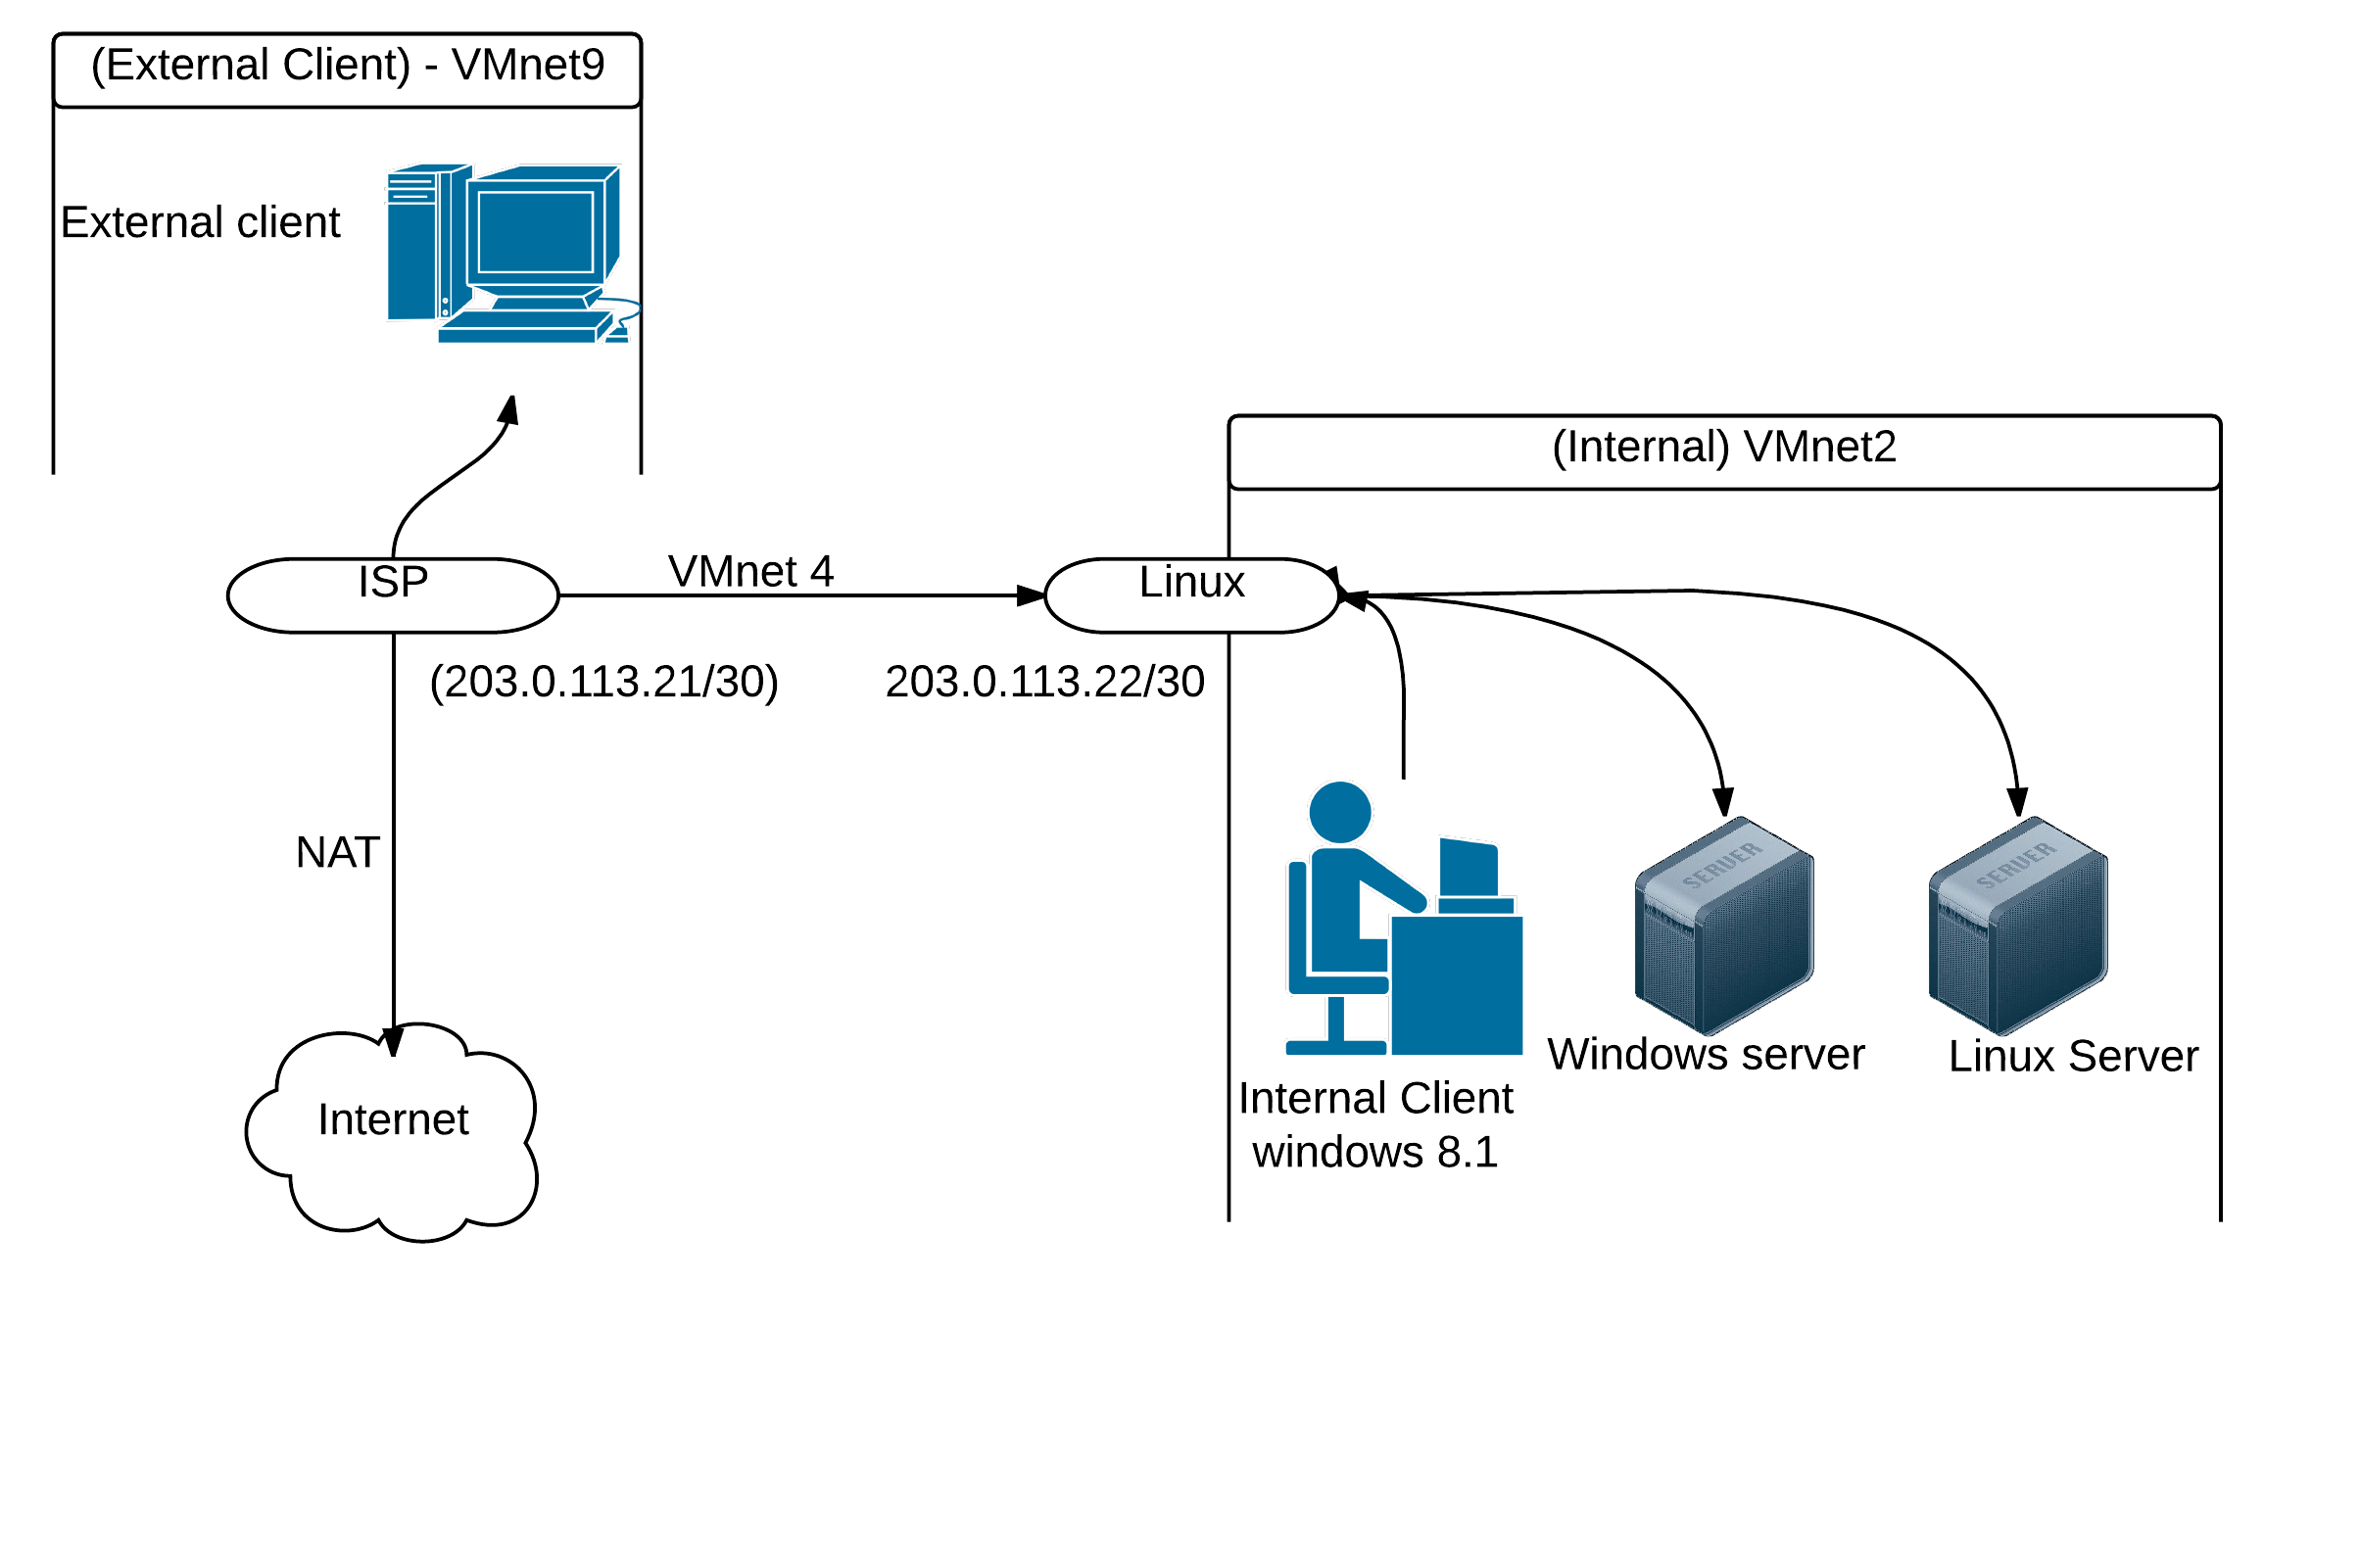
\includegraphics[width=1\linewidth]{./network}
\caption[Figure over network in Lab 1]{The network as it should be setup in Lab 1.}
\label{fig:network}
\end{figure}
You have been given the the task to setup a newly founded company's network. In \figurename \ref{fig:network} you should see how the network should look when you are done with lab 1.

The topology contains one Linux server, one Windows Server 2012 R2 , one Linux machine as a router and one Windows 8.1 client on the internal. all of these should be connected to VMnet2. The Linux router is also connected to the ISP Gateway with the VMNet 4.
We also have an external client on VMNet 9.

\section{Requirements}
\label{tasks}
Aside from the network sketch there are some requirements the company have but on these.

\begin{itemize}
    \item All machines should:
    \begin{itemize}
        \item have static ip-addressing, the addresses is up to you to decide but you should be able to motivate your choice. 
	\item should have internet access using the linux router.
	\item shoule be able to ping eachother on the their respective VMNet.
        \item have proper firewall rules. This includes both the linux and windows machines.
    	\item Have a proper naming convention.
    \end{itemize}
	\item Specific machinerequirements:
    \begin{itemize}
        \item \textbf{ISP Gateway}
        \begin{itemize}
		\item This is the only machine that you will not install yourself, it is a predefined machine that you will make a linked clone of.
        	\item The template is located at \textbf{c:\textbackslash VirtualLabs\textbackslash Files\textbackslash Templates\textbackslash ISP Gateway Template\textbackslash }
        \end{itemize}

        \item \textbf{Linuxrouter}
        \begin{itemize}
		\item should have two network interfaces, one for VMnet 4 pointing to the ISP Gateway and one for the local Server LAN VMnet2.
            	\item The ISP pointing interface should be configured according to the network sketch in \figurename \ref{fig:network}, \textit{Observe! To be able to lookups it needs to use the ISP Gateways DNS server.}
        \end{itemize}
        
        \item \textbf{Other OS}
        \begin{itemize}
		\item Only be connected to their respective VMNet.
        \end{itemize}
        
    \end{itemize}
\end{itemize}

\section{Workenviroment}
\label{enviroment}

You will be using VMware Workstation to be able to accomplish this lab. You will only use templates for the ISP Gateway in this lab. The rest is up to you to construct from isofiles.
 
To be able to start this laboration you need to have signed up for MSNDAA and a labbgroup. When you have done this it takes up to a workday before you are put into the system.

\paragraph{ISO} At your disposal there are \win{2012 R2} och Windows 8.1 ISOs på 
C:\textbackslash VirtualLabs\textbackslash Files\textbackslash MSDNAA\textbackslash Operating Systems
%kolla upp var imorgon.
\end{document}
